\documentclass[10pt,a3paper]{article}
\usepackage{scalefnt}
\usepackage{geometry}
\usepackage{pdflscape}
\usepackage{tikz}
\usepackage{mathtools}
\usetikzlibrary{calc}
%\usetikzlibrary{positioning}
%\usetikzlibrary{intersections}
\pagestyle{empty}
\tikzset{x=1cm,y=1cm}

\def\scalesize{8}
\def\x{-\scalesize}
\def\z{\scalesize}
\def\y{0.7*\scalesize}
\def\theta{30}
%\def\yh{0.5*\scalesize}
%\def\yv{0.5*\scalesize}
\def\aboffset{0.2}



\begin{document}
\def\marginsize{0.5cm}
\def\xmax{20}
\def\ymax{14}
\def\xmin{-\xmax}
\def\ymin{-\ymax}
\newgeometry{margin=\marginsize}
\begin{landscape}
\scalefont{1.5}
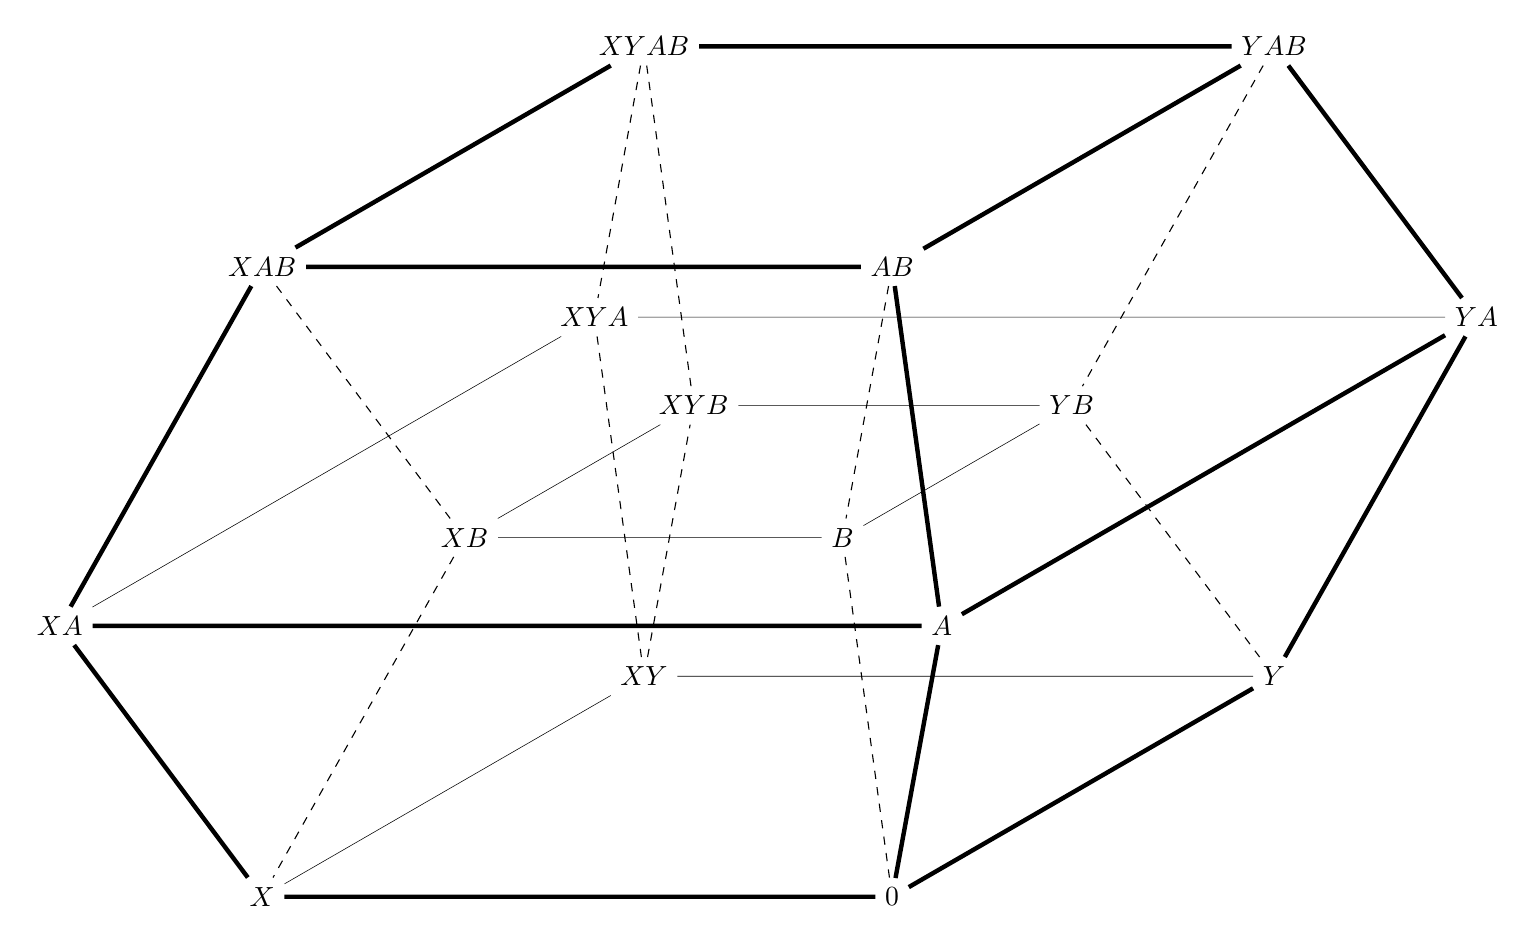
\begin{tikzpicture}

%% Draw a background grid with numbered axes, all in faint grey
%\tikzset{BkgGrid/.style={gray, opacity = 0.5}};
%
%\draw[BkgGrid, help lines] (\xmin,\ymin) grid (\xmax,\ymax);
%\foreach \x in {\xmin,...,\xmax}
%	\draw [BkgGrid] (\x,0pt) -- (\x,-3pt)
%	node[BkgGrid, anchor=north] {\x};
%\foreach \y in {\ymin,...,\ymax}
%	\draw [BkgGrid] (0pt,\y) -- (-3pt,\y) 
%	node[BkgGrid, anchor=east] {\y}; 
		
\node (0) at (0,0) {$0$};	
\node (X) at ($(0)+(\x,0)$) {$X$};	
\node (Z) at ($(0)+(0,\z)$) {$AB$};	
\node (XZ) at ($(0)+(\x,\z)$) {$XAB$};	

\node (Y) at  ($(0)+(\theta:\y)$) {$Y$};	
\node (XY) at ($(X)+(\theta:\y)$) {$XY$};	
\node (ZY) at ($(Z)+(\theta:\y)$) {$YAB$};	
\node (XYZ) at ($(XZ)+(\theta:\y)$) {$XYAB$};	

\draw[ultra thick] (0) -- (X)  (XZ) -- (Z)  (0) -- (Y)  (ZY) -- (XYZ) -- (XZ) ;
\draw[ultra thick] (Z) -- (ZY);
\draw[very thin] (X) -- (XY) -- (Y);
%\draw[thick] (XY) -- (XYZ);


\coordinate (half0-Z) at ($(0)+(0,0.5*\z)$);
\coordinate (halfXY-XYZ) at ($(XY)+(0,0.5*\z)$);

\coordinate (halfY-ZY) at ($(Y)+(0,0.5*\z)$);
\coordinate (halfX-XZ) at ($(X)+(0,0.5*\z)$);

%\draw[dashed] (half0-Z) -- (halfXY-XYZ); 
\node (T) at ($(half0-Z)!-\aboffset!(halfXY-XYZ)$) {$A$};
\node (S) at ($(half0-Z)!\aboffset!(halfXY-XYZ)$) {$B$};
\node (P) at ($(half0-Z)!1-\aboffset!(halfXY-XYZ)$) {$XYB$};
\node (Q) at ($(half0-Z)!1+\aboffset!(halfXY-XYZ)$) {$XYA$};

%\draw[dashed] (halfY-ZY) -- (halfX-XZ);
\node (F) at ($(halfY-ZY)!-\aboffset!(halfX-XZ)$) {$YA$};
\node (G) at ($(halfY-ZY)!\aboffset!(halfX-XZ)$) {$YB$};
\node (H) at ($(halfY-ZY)!1-\aboffset!(halfX-XZ)$) {$XB$};
\node (I) at ($(halfY-ZY)!1+\aboffset!(halfX-XZ)$) {$XA$};


\draw[ultra thick] (0) -- (T) -- (Z);
\draw[dashed] (Z) -- (S) -- (0);
\draw[ultra thick] (X) -- (I) -- (XZ);
\draw[dashed] (XZ) -- (H) -- (X);
\draw[ultra thick] (Y) -- (F) -- (ZY); 
\draw[dashed] (ZY) -- (G) -- (Y);
\draw[dashed] (XY) -- (P) -- (XYZ) -- (Q) -- (XY);

\draw[very thin] (H) -- (P) -- (G) -- (S) -- (H);
\draw[very thin] (I) -- (Q) -- (F);
\draw[ultra thick] (F) -- (T) -- (I);

\end{tikzpicture}
\end{landscape}
\end{document}